\documentclass[portrait,a0]{a0poster}
\usepackage{color,multicol}
\usepackage[english]{babel}
\usepackage[utf8]{inputenc}
\usepackage[T1]{fontenc}
\usepackage{siunitx}
\usepackage{graphicx}
\usepackage{booktabs}
\usepackage[round]{natbib}
\usepackage[font=small]{caption}
\usepackage{lmodern}
\usepackage[overload]{textcase}
\usepackage{setspace}
\usepackage{float}
\usepackage{titlesec}
\usepackage{lipsum} % Lorem ipsum generator
\usepackage{caption}

\columnsep = 50pt % change this for separation of the columns

\definecolor{facultyColor}{cmyk}{0,.37,.88,.02} % faculty of science
\definecolor{gray}{cmyk}{.13,.05,0,.25}

\titleformat{\section}[hang]
{\LARGE\usefont{T1}{phv}{bx}{n}\color{facultyColor}} % format
{} % label
{0pt} % sep
{\MakeUppercase} % before-code

\begin{document}

\large

%\vspace*{\fill} %some more marginal up

%\begin{minipage}[t]{0.98\linewidth} % The first minipage for the logo & title
%\vspace{0pt} % A trick to align the parallel minipages on top

%\vspace{0.008\linewidth} % Increase the top margin
%\begin{multicols}{2} 
\begin{minipage}[t]{.4\linewidth} % logo
\vspace{0pt} % Alingns the parallel minipages on top

\includegraphics[height=0.35\linewidth]{HYlogo_fac_text-en}
\hspace{50pt}
%\includegraphics[width=0.35\linewidth]{division}
\end{minipage} % no empty line before the next begin

\vspace{-12cm}
\begin{minipage}[t]{.98\linewidth} % logo
\vspace{0pt} % Alingns the parallel minipages on top
\begin{flushright}
\begin{spacing}{5}
%{\usefont{T1}{phv}{bx}{n}\textcolor{facultycolor}{\MakeUppercase{Faculty of Science}} \MakeUppercase{}} 
{\Huge\usefont{T1}{phv}{bx}{n}\textcolor{black}{\MakeUppercase{Helsingin Yliopisto}} \MakeUppercase{}}\\
{\Huge\usefont{T1}{phv}{bx}{n}\textcolor{black}{\MakeUppercase{Helsingfors Universitet}} \MakeUppercase{}}\\
{\Huge\usefont{T1}{phv}{bx}{n}\textcolor{black}{\MakeUppercase{University of Helsinki}} \MakeUppercase{}}\\
{\Huge\usefont{T1}{phv}{bx}{n}\textcolor{facultyColor}{\MakeUppercase{Matemaattis-Luonnontieteellinen tiedekunta}} \MakeUppercase{}}\\
{\Huge\usefont{T1}{phv}{bx}{n}\textcolor{facultyColor}{\MakeUppercase{Matematisk-Naturvetenskapliga fakulteten}} \MakeUppercase{}}\\
{\Huge\usefont{T1}{phv}{bx}{n}\textcolor{facultyColor}{\MakeUppercase{Faculty of Science}} \MakeUppercase{}}\\
\end{spacing}
\end{flushright}
\hspace{50pt}

\end{minipage} % no empty line before the next begin

%\end{minipage}

%\end{multicols}


\begin{multicols}{2} 
\begin{minipage}[t]{1.4\linewidth}
\vspace{10pt}
\begin{flushleft}
\begin{spacing}{5}
%\begin{center}
% Highlight two first words of the title with the faculty color
{\Huge\usefont{T1}{phv}{bx}{n}\textcolor{gray}{\MakeUppercase{How a Pseudonym Based Solution to Defeat IMSI-catchers Opens a Vulnerability to} DoS} \MakeUppercase{}} \\

%\end{center}
\end{spacing}
\end{flushleft}
\end{minipage}

\begin{minipage}[t]{.95\linewidth} % title
\vspace{-90pt} % Alingns the parallel minipages on top
\begin{flushright}
\textsf{\bfseries
Mohsin Khan \\
Kimmo Järvinen\\
Philip Ginzboorg\\
Valtteri Niemi\\
} % Text size for a1 posters
\textcolor{gray}{\textsf{\bfseries{Department of Computer Science\\University of Helsinki}}}
\end{flushright}
\end{minipage}
\end{multicols}

%\end{minipage}
\vspace{-70pt}
%\vfill % some more marginal between header and text
\noindent\makebox[\linewidth]{\rule{\paperwidth}{5pt}}

\begin{multicols}{2} % change this for different number of columns


\section{IMSI-Catchers}
\begin{enumerate}
\item A user equipment (UE) has to identify itself before attaching to a serving network (SN)
\item Before identification, there is no agreed security context in between a UE and the SN
\item As a result, whenever an SN inquires a UE's IMSI, the UE responds with IMSI in cleartext
\end{enumerate}

\begin{center}
\begin{minipage}[t]{0.9\linewidth} % logo
\vspace{.25cm} % Alingns the parallel minipages on top
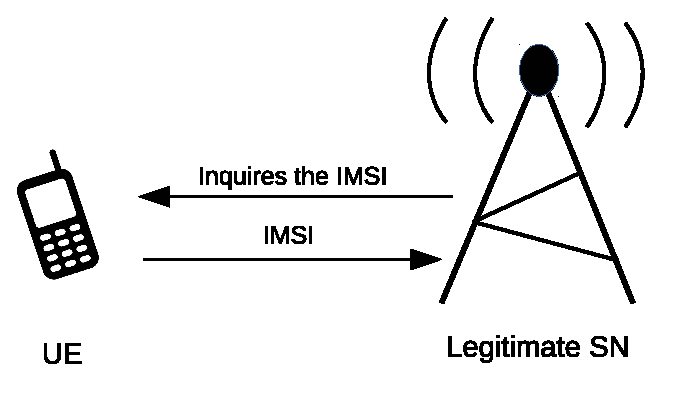
\includegraphics[width=.8\linewidth]{IMSI-catcher.eps}
\hspace{0pt}
\vspace{.25cm} % Alingns the parallel minipages on top
\end{minipage} 
\end{center}

\noindent
An IMSI-catcher is a fake SN that impersonates a legitimate SN. An IMSI-catcher sends an IMSI inquiry to a UE. According to above protocol, the UE responds with the IMSI in cleartext.

\begin{center}
\begin{minipage}[t]{0.9\linewidth} % logo
\vspace{.25cm} % Alingns the parallel minipages on top
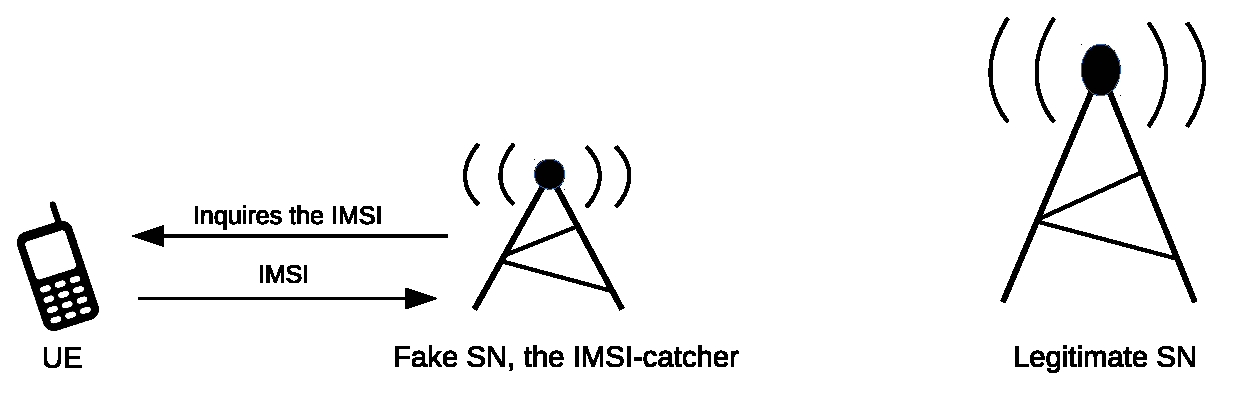
\includegraphics[width=1\linewidth]{IMSI-catcher1.eps}
\hspace{0pt}
\vspace{.25cm} % Alingns the parallel minipages on top
\end{minipage} 
\end{center}


\begin{itemize}
\item IMSI-catchers violate identity privacy and UEs need to be protected from them
\item IMSI-looking temporary identifiers known as pseudonyms are proposed \citep{Ginzboorg_Niemi_2016,Norrman_Naslund_Dubrova_2016,CCS15,SSR15} to defeat IMSI-catchers
\item We show that all of them defeat the IMSI-catchers but open a vulnerability to a DoS attack
\item We choose \citep{CCS15} paper to demonstrate our attack. Similar attack can be mounted on others
\end{itemize}


\section{Pseudonym Based Solution}
In \citep{CCS15}, the pseudonym based solution works as follows. Every user UE is given IMSI-looking temporary identifiers we call pseudonyms. When a network inquires for IMSI, the UE responds with a pseudonym instead of IMSI.

\begin{center}
\begin{minipage}[t]{0.9\linewidth} % logo
\vspace{.25cm} % Alingns the parallel minipages on top
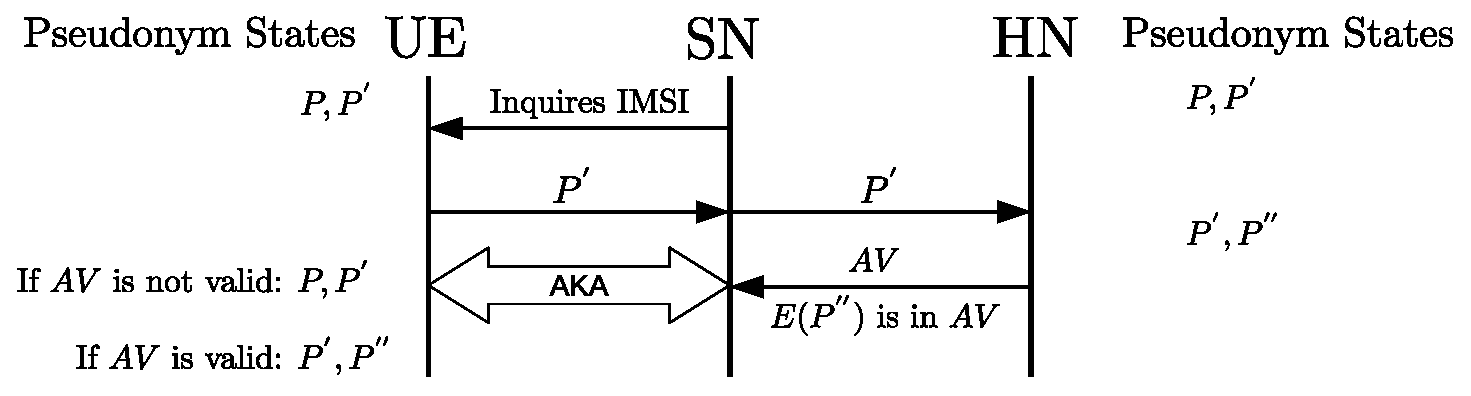
\includegraphics[width=1\linewidth]{ccs_solution.eps}
\hspace{0pt}
\vspace{.25cm}
\end{minipage}
\end{center}

\begin{enumerate}
\item A pair $P,P^{'}$ of pseudonyms is involved with every UE
\item Whenever a network inquires for IMSI, the UE responds either with $P$ or $P^{'}$
\item If UE responds with $P$, the pseudonym states do not change
\item \label{item:weakness} If UE responds with $P^{'}$, the pseudonym states change from $P,P^{'}$ to $P^{'},P^{''}$
\item $P^{''}$ is generated at home network (HN)
\item $P^{''}$ is encrypted and piggybacked with the authentication vector ($AV$)
\item Nobody except the UE can know $P^{''}$ until the UE uses $P^{''}$ as a response of an IMSI inquiry
\end{enumerate}

\subsection*{Weakness}This solution has a weakness in item \ref{item:weakness}. The HN does not authenticate the origin of the message that carries a pseudonym from UE to HN and generates a new pseudonym $P^{''}$ whenever it observes the pseudonym $P^{'}$. This fact can be exploited to mount a DoS attack.

\section{A D\MakeLowercase{o}S Attack}
The DoS attack forces the pseudonym state of a user in HN to go to a state which is completely different from the pseudonym state of the user in its UE. Consequently the UE will not be able to identify itself sucessfully anymore to the network. The attack is as follows:
\begin{enumerate}
\item \label{send_fake_pseudonym} A fake UE (FUE) sends a pseudonym $q_1$ to a legitimate SN and SN forwards $q_1$ to the HN
\item \label{q_equal_pseudonym} Let $P_x,P_x^{'}$ be the pseudonym state of a user $x$. Let us assume that $q_1=P_x^{'}$. The pseudonym state at HN will be updated to $P_x^{'},P_x^{''}$
\item The FUE then sends $q_2$ to the legitimate SN and the SN forwards $q_2$ to respective HN
\item Let us assume that $q_2=P_x^{''}$. The pseudonym state at HN will be updated to $P_x^{''},P_x^{'''}$
\item Pseudonym state for the user $x$ is still \textcolor{red}{$P,P^{'}$} in UE, but \textcolor{red}{$P_x^{''},P_x^{'''}$} in HN
\end{enumerate}

\begin{center}
\begin{minipage}[t]{0.9\linewidth} % logo
\vspace{.25cm} % Alingns the parallel minipages on top
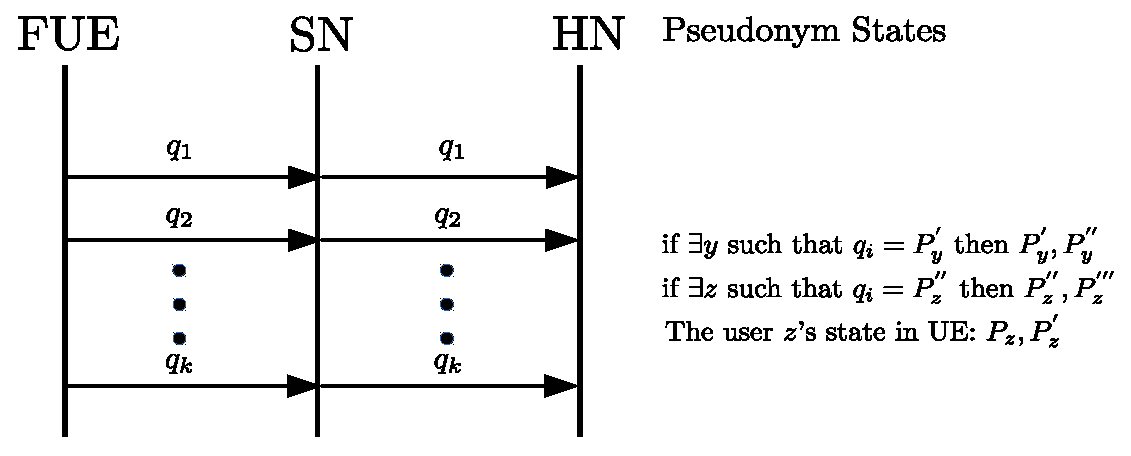
\includegraphics[width=1\linewidth]{attack.eps}
\hspace{0pt}
\vspace{.25cm} % Alingns the parallel minipages on top
\end{minipage} 
\end{center}

\begin{itemize}
\item Now if $k$ is a large number, we can expect that there would be many users $x$ for which $\exists i,j$ such that $1 \leq i < j \leq k$, $q_i=P_x^{'}$ and $q_j=P_x^{''}$
\item  All such users $x$ would then have different pseudonym states in their UE than in the HN
\item If an attacker mounts such an attack in a distriubted fashion by employing hundreds of FUEs, the whole IMSI space ($10^{10}$) can be exhausted twice within few hours and consequently the whole network will go out of service
\item This attack can be used in cyberwarfare, terrorism or blackmailing the network operator
\end{itemize}

\section{Solution}
\begin{enumerate}
\item Authenticating the message that carries a pseudonym from the UE to the SN using MAC 
\begin{enumerate}
\item The HN knows if the pseudonym is sent by the user associated with the pseudonym
\item This solution works in 5G but doesn't work in 3G or 4G  
\end{enumerate}
\item Use existing messages to confirm HN that UE has received the new pseudonym
\begin{enumerate}
\item Location update message sent by an SN to the HN can be used 
\item This solution introduces a new DoS attack by introducing a man in the middle (MITM)
\item An MITM can possibly be detected using Security mode command (SMC) 
\end{enumerate}
\end{enumerate}

\begin{center}
\begin{minipage}[t]{0.9\linewidth} % logo
\vspace{0cm} % Alingns the parallel minipages on top
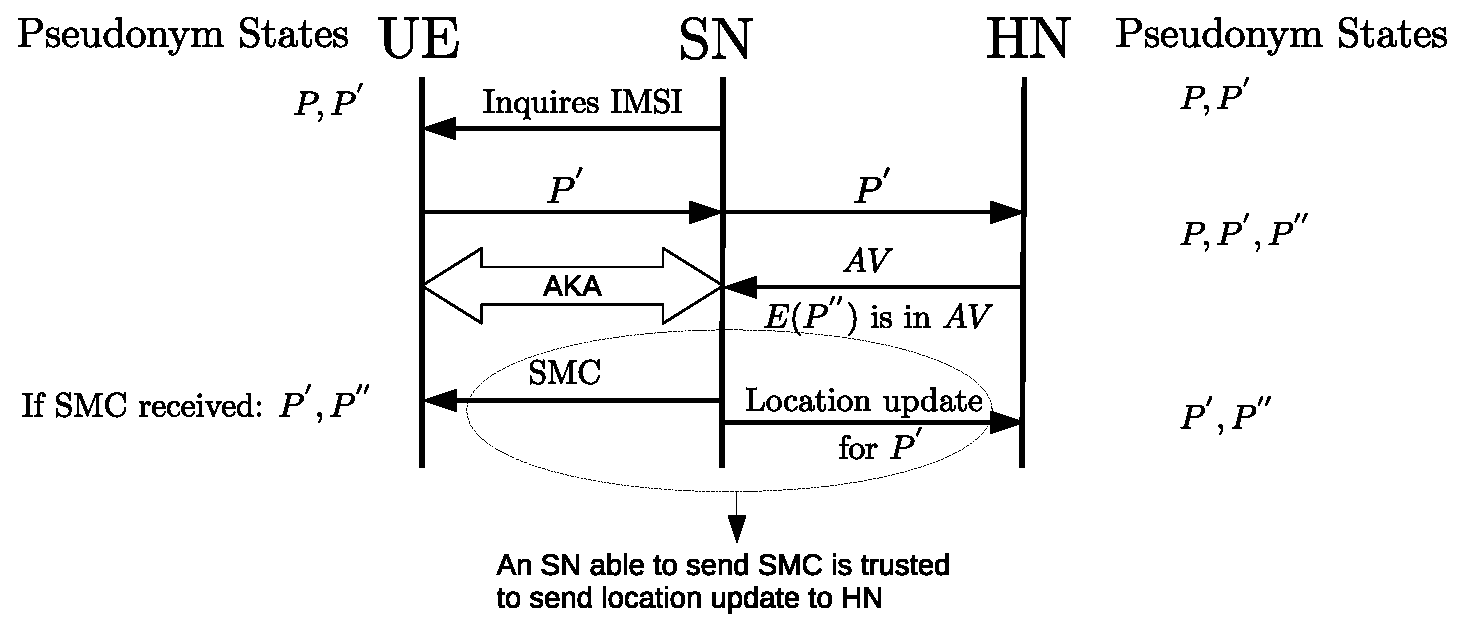
\includegraphics[width=1\linewidth]{solution.eps}
\hspace{0pt}
\vspace{0cm} % Alingns the parallel minipages on top
\end{minipage} 
\end{center}

\noindent
If no location update is received for pseudonym $P^{'}$ but $P^{''}$ is observed at the HN, the new pseudonym generated by the HN is still $P^{''}$. It is trusted that if an SN is capable of sending a valid SMC to the UE after an AKA, the SN will send the location update to the HN.

\normalsize

\bibliographystyle{abbrvnat}
\bibliography{ref}

\end{multicols}

\vfill % some more marginal in the end

\begin{minipage}[t]{0.9\linewidth} % footer
\footnotesize
\color{gray}{\textsf{\textbf{The {\LaTeX} template by Jussi Tiira used in this poster is licensed under a Creative Commons Attribution 4.0 International License.}}}
\end{minipage}


\end{document}
